\documentclass[a4paper]{article}

% Packages
\usepackage[left=25mm, top=30mm,]{geometry}
\usepackage{graphicx}
\usepackage{float}
\usepackage{siunitx}
\usepackage{listings}
\usepackage{physics}
\usepackage[dutch]{babel}
\usepackage{fixltx2e}

\renewcommand{\lstlistingname}{Algoritme}
\renewcommand{\lstlistlistingname}{Lijst van algoritmen}

\lstset{
	language=Matlab,
	captionpos=b,
	frame=single,
	numbers=left,
	numberstyle=\tiny\color{{rgb}{0.5,0.5,0.5}},
	showstringspaces=false,
}

\usepackage{hyperref}
\hypersetup{pdfborder={0 0 0}}

% Commands and stuff
\newcommand{\opgave}[1]{\subsection{Opgave #1}}

% Title Page stuff
\title{Practicum Numerieke Modelering en Benadering}
\author{Wim Kunnen, r0629332 \\ Bo Kleynen, r0624034}
\date{zondag 15 april 2018 }

% Actual document
\begin{document}

\begin{titlepage}
\maketitle
\thispagestyle{empty}
\end{titlepage}


% Table of Contents
\pagenumbering{roman}
\setcounter{page}{1}
\tableofcontents
\cleardoublepage

% List of figures
\listoffigures
\addcontentsline{toc}{section}{\numberline{} Lijst van tiguren}

% List of Tables
\listoftables
\addcontentsline{toc}{section}{\numberline{} Lijst van tabellen}

\lstlistoflistings
\addcontentsline{toc}{section}{\numberline{} Lijst van algoritmen}

\cleardoublepage



\pagenumbering{arabic}
\setcounter{page}{1}

% PDE stuff
\section{Partial Differential Equations}\label{sec:PDE}
Het eerste deel behandelt het zoeken van een benaderende oplossing voor de Poisson vergelijking met als domein het eenheidsvierkant en gegeven Dirichlet randvoorwaarden.

\begin{equation}\label{eq:poisson}
	\pdv[2]{u(x,y)}{x} + \pdv[2]{u(x,y)}{y} = f(x,y) \quad met (x,y) \in D = [ \, 0,1 ]\, \times [ \, 0,1 ]\,
\end{equation}
Met randvoorwaarden van de vorm:
\begin{equation}\nonumber
	u_w(y) = u(0,y), \quad u_o = u(1,y), \quad u_z = u(x,0) \quad en \quad u_n = u(x,1)
\end{equation}



% OPGAVE 1
\opgave{1: Implementatie en controle}\label{sec:oef1}
De implementatie van het gegeven algoritme
\lstinputlisting[caption=PDE]{../Matlab/PDE.m}
De correctheid van de implementatie werd geverifieerd door het oplossen van \ref{eq:poisson} voor de volgende gevallen:
\begin{itemize}
	\item $\nabla^2u(x,y)=0$ met randvoorwaarden $u_w(y)=u_o(y)=u_z(x)=u_n(x)=0$ met als exacte oplossing $u(x,y) = 1$
	\item $\nabla^2u(x,y)=0$ met randvoorwaarden $u_w(y)=1+y$, $u_o(y)=2+y$, $u_z(x)=1+x$ en $u_n(x)=2+x$ met als exacte oplossing $u(x,y) = 1 + x + y$
	\item $\nabla^2u(x,y)=4$ met randvoorwaarden $u_w(y)=y^2$, $u_o(y)=1+y^2$, $u_z(x)=x^2$ en $u_n(x)=1+x^2$ met als exacte oplossing $u(x,y) = x^2 +y^2$
\end{itemize}


% OPGAVE 2
\opgave{2: Fouten en tijdsduur}\label{sec:oef2}
In deze sectie bekijken we de nauwkeurigheid van de implementatie aan de hand van de volgende vergelijking:
\begin{equation}
	\nabla^2u(x,y) = e^{x+y}
\end{equation}
met randvoorwaarden:
\begin{equation}
	u_w(y)=e^y, \quad u_o(y)=e^{1+y}, \quad u_z(x)=e^x, \quad u_n(x)=e^{1+x}
\end{equation}
en exacte oplossing
\begin{equation}
	u(x,y) = e^{x+y}
\end{equation}

Tabel \ref{tab:fouten} toon de maximale fout en de rekentijd voor een aantal waarden van N.

% Tabel met fouten
\begin{table}[H]
	\centering
	\begin{tabular}{l c r}
		N & Maximale fout & Tijd [seconde] \\ \hline
		8 & \num{1.6118e-04} & 0.002915 \\
		16 & \num{4.5544e-05} & 0.000922 \\		
		32 & \num{1.2136e-05} & 0.000538 \\
		64 & \num{3.1300e-06} & 0.000827 \\
		128 & \num{7.9485e-07} & 0.005202 \\
		256 & \num{2.0027e-07} & 0.013696 \\
		512 & \num{5.0268e-08} & 0.039208 \\
		1024 & \num{1.2605e-08} & 0.231955
	\end{tabular}
	\caption{Tabel met fouten in functie van discretisatie}
	\label{tab:fouten}
\end{table}

Een voorzichtige schatting leert ons dat de maximale fout $\mathcal{O}(\frac{3}{2}N)$ is.

% OPGAVE 3
\opgave{3: Plot}\label{sec:oef3}
Tot slot werd er gevraagd om de Poissonvergelijking op te lossen voor volgend $f(x,y)$. 
\begin{equation}
f(x,y) =
  \begin{cases}
    -100       & \quad \text{als } (x,y) \in D = [ \, 0.4,0.6 ]\, \times [ \, 0.4,0.6 ]\,\\
    0  & \quad \text{anders }
  \end{cases}
\end{equation}
Met randvoorwaarden:
\begin{equation}
	u_w(y) = 3, \quad u_o = 2, \quad u_z = 2+\sin{(\frac{\pi}{2}x)} \quad en \quad u_n = 1
\end{equation}
Onderstaand stuk code toont het matlab script gebruikt om dit randwaardeprobleem op te lossen.
\lstinputlisting[language=Matlab, caption=script opgave 3]{../Matlab/opgave3.m}

Figuur \ref{fig:Contour3} toont de contour plot en figuur \ref{fig:Plot3} het 3 dimensionale oppervlak van de benaderende oplossing.
\newpage
% Contour figuur
\begin{figure}[H]
	\begin{center} 
		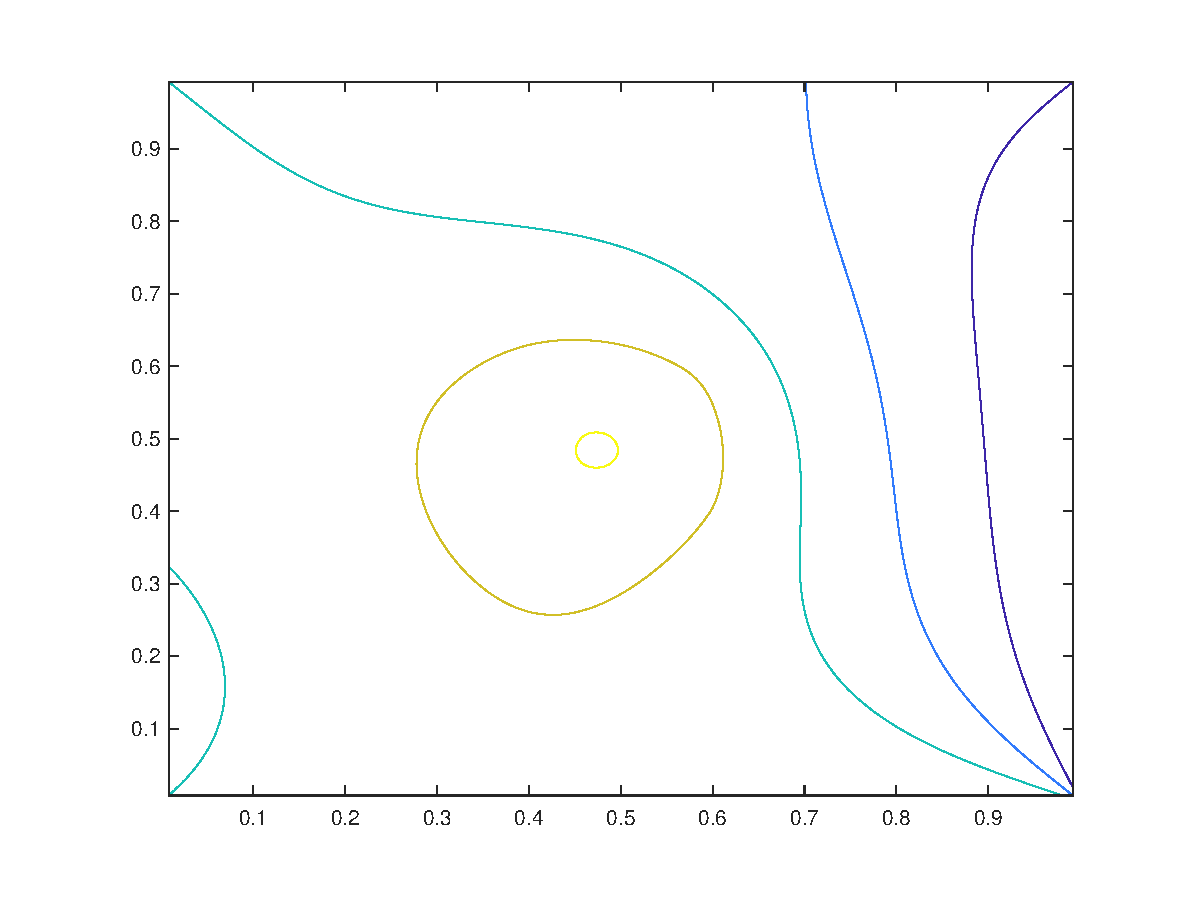
\includegraphics[width=0.7\textwidth]{Contour3.eps}
	\end{center}
	\caption{De contour plot voor Opgave 3.}
	\label{fig:Contour3}
\end{figure}

% Plot
\begin{figure}[H]
	\begin{center} 
		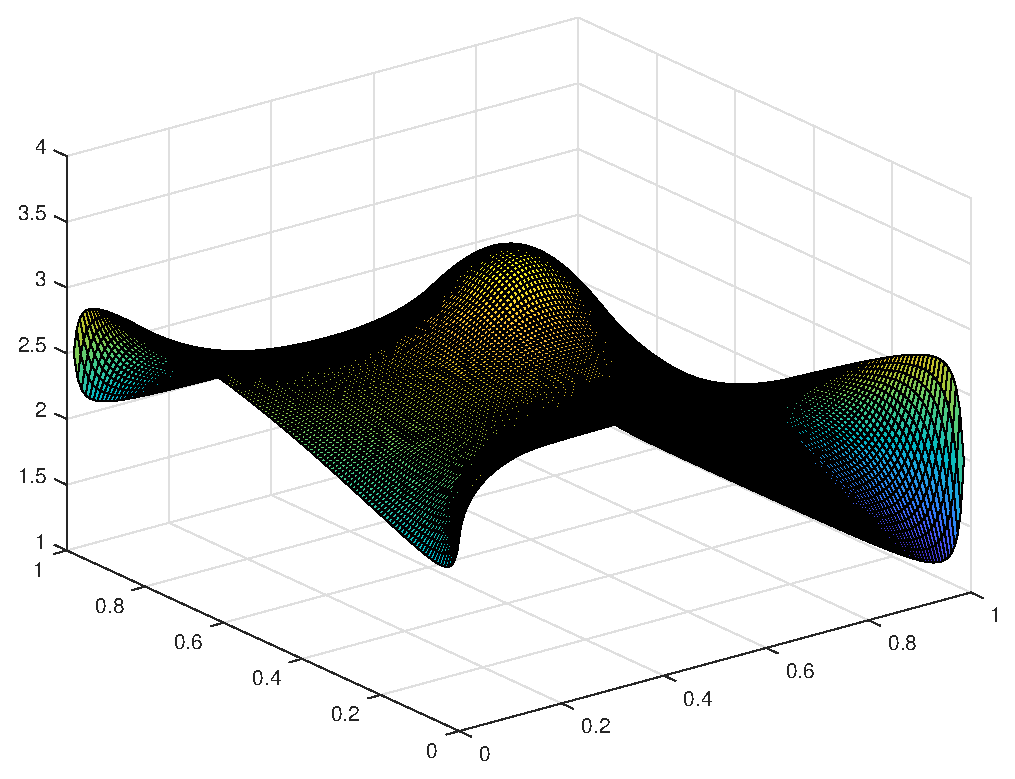
\includegraphics[width=1\textwidth]{Plot3.eps}
	\end{center}
	\caption{De plot voor Opgave 3.}
	\label{fig:Plot3}
\end{figure}
\newpage

% Splines stuff
\section{Splines}\label{sec:splines}
Dit deel behandelt het opstellen van een kleinste-kwadraten benadering met behulp van splinefuncties. Eerst komt de implementatie van een effici\"ente methode voor het opstellen van een kleinste-kwadraten spline benadering in matlab aan bod daarna volgt de implementatie van het algoritme van de Boor om deze benadering te evalueren en tot slot een bespreking van opgaven 5 tot en met 7.

% OPGAVE 4
\subsection{Implementatie van de algoritmen}
\subsubsection{Opstellen van de kleinste-kwadraten benadring}
Uitgaande van het algoritme in sectie 2.2 van de opgave stellen we volgende tabel op om de matrix M te bepalen, voor $x \in [t_j, t_{j+1}]$ en $l=1, 2, ... k$ met $k$ de graad van de spline benadering.
\begin{table}[H]
	\centering
	\begin{tabular}{| c c c c c c c  |}
		\hline
		& & & & & & $N_{j-k,k+1}(x)$ \\
		& & & & & . & $N_{j-k+1,k+1}(x)$ \\
		& & & & $N_{j-l,l+1}(x)$ & $\hdots$ & $N_{j-k+2,k+1}(x)$ \\
		& & & . & $\vdots$  & & $\vdots$\\
		& & $N_{j-2,3}(x)$ & $\hdots$ & $N_{j-\gamma+1,l+1}(x)$ & $\hdots$ & $N_{j+2,k+1}(x)$   \\
		& $N_{j-1,2}(x)$ & $N_{j-1,2}(x)$ & $\hdots$ & $\vdots$ &  &$N_{j+1,k+1}(x)$ \\
		$N_{j,1}(x) = 1$ & $N_{j,2}(x)$ & $N_{j,3}(x)$ & $\hdots$ & $N_{j,l+1}(x)$ & $\hdots$ & $N_{j,k+1}(x)$ \\ 
		\hline
	\end{tabular}
\end{table}
In de $l$-de kolom (beginnend vanaf 0) staan de functiewaarden van alle B-splines van graad $l$, die verschillend zijn van 0 in het punt x. 
$N_{j-l,l+1}(x)$ hangt enkel af van $N_{j-l+1,l}(x)$ en wordt daarom telkens als eerste bepaald, zo kunnen de  waarden van opeenvolgende $N_{\alpha,l+1}(x)$ telkens op de juiste plaats in de matrix M opgeslagen worden. Vervolgens worden de waarden van $N_{j-\gamma+1,l+1}(x)$ bepaald voor $\gamma$ gaande van $1$ tot en met $k-1$ en tot slot de waarde van $N_{j,l+1}(x)$ die enkel afhangt van $N_{j,l}(x)$. Om het programma wat overzichtelijker te houden en de hoeveelheid rekenwerk minimaal te houden wordt volgende substitutie doorgevoerd: $i=j-\gamma$ met $i$ gaande van $j-l+1$ tot en met $j-1$.
\newpage
\lstinputlisting[language=Matlab, caption=kkbSpline]{../Matlab/kkbSpline.m}
\newpage

\subsubsection{Algoritme van de Boor}
Gegeven een een splinefunctie die een lineaire combinatie is van $n+k$ B-splines
\begin{equation}\label{eq:deboor}
	s(x) = \sum\limits_{i=-k}^{n-1} c_iN_{i, k+1}(x)
\end{equation}
Kan deze zeer effici\"ent ge\"evalueerd worden, gebruik makend van het algoritme van de Boor:
Zij $x\in[t{j}, t_{j+1})$ dan geldt $s(x)=c_{j}^{[k]}$ met $c_i^{[0]} = c_i$ en $c_i^{[r]}$ wordt gevonden uit:
\begin{equation}\label{eq:deboorcoef}
	c_i^{[\, r]\, } = \alpha_{i,r} c_i^{[\, r-1]\, } + (1-\alpha_{i,r})c_{i-1}^{[\, r-1]\, } \quad met \quad \alpha_{i,r} = \frac{x-t_i}{t_{i+k+1-r}-t_i}
\end{equation}

Per waarde van $r$ worden de $c_i^{[\, r]\, }$ bepaald volgens afnemende $i$ dus voor $i$ gaande van $j$ tot en met $j-k+r$ voor $r$ gaande van $1$ tot en met $k$, op die mannier kan de waarde van $c_i^{[\, r]\, }$ op dezelfde plaats in het computergeheugen opgeslagen worden als $c_i^{[\, r-1]\, }$.

\lstinputlisting[language=Matlab, caption= de Boor]{../Matlab/deBoor.m}


% OPGAVE 5
\opgave{5: Illustratie correctheid}\label{sec:oef5}
Ter illustratie van de correctheid van de implementatie van het algoritme van de Boor toont figuur \ref{fig:splines}, 5 kubische splines (graad k = 3).

%Plot Splines
\begin{figure}[H]
	\begin{center} 
		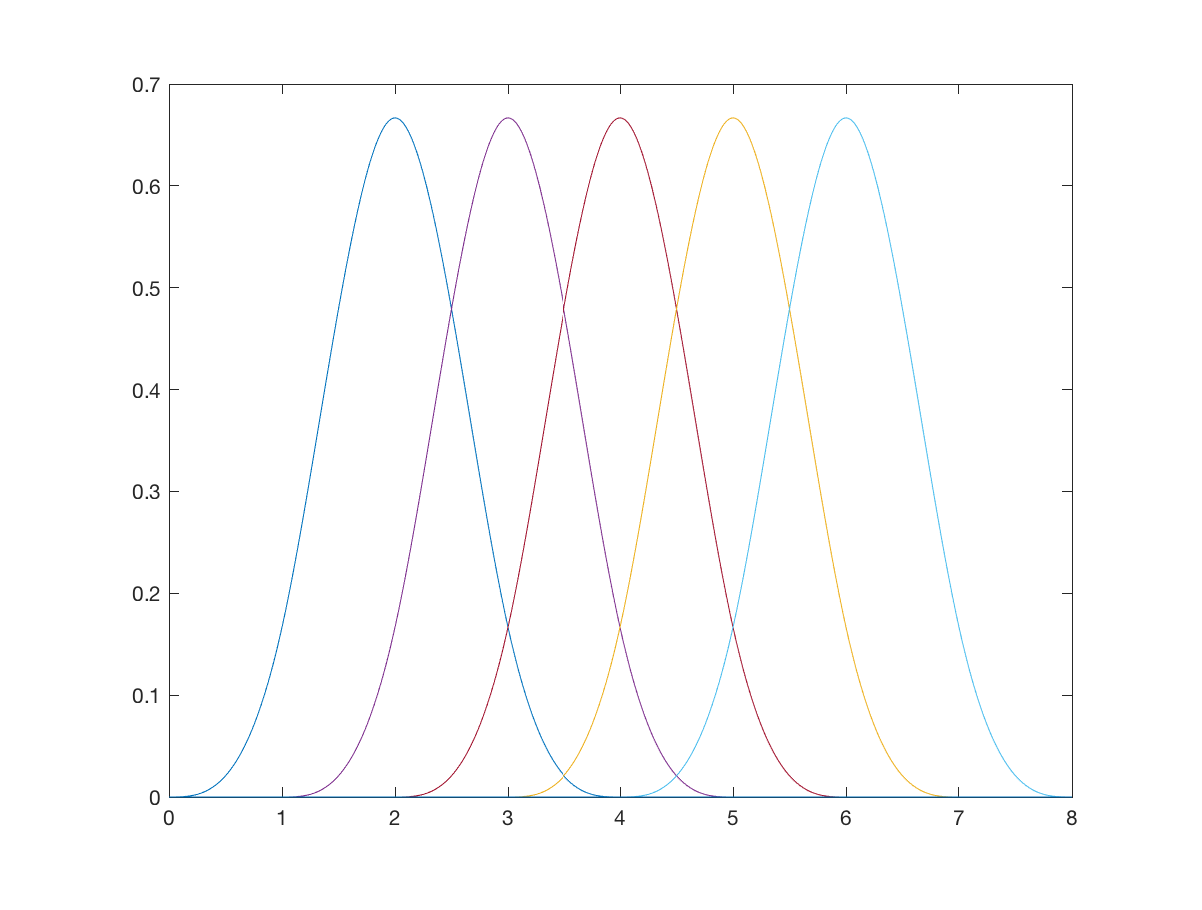
\includegraphics[width=0.6\textwidth]{BSplines.eps}
	\end{center}
	\caption{Kubische B-splines voor Opgave 5.}
	\label{fig:splines}
\end{figure}
\newpage

% OPGAVE 6
\opgave{6: Ligging knooppunten}\label{sec:oef6}
Ter illustratie van het effect van de ligging van de knooppunten werd de rechthoekige puls (\ref{eq:rect}) benaderd (figuur  \ref{fig:rectan}).

\begin{equation}
f(x) =
  \begin{cases}
    1       & \quad \text{als } -0.5 < x < 0.5\\
    0  & \quad \text{anders }
  \end{cases}
  \label{eq:rect}
\end{equation}

We namen eerst een benadering op basis van 20 equidistante knooppunten op het interval [-1,1]. Deze werd op de figuur getekend (blauw) samen met de rechthoekpuls (rood). \\

Daarna werd de rechthoekpuls benaderd door middel van 20 knooppunten die dicht bij de flanken van de puls te kiezen. Deze flanken vari\"eren zeer sterk, waardoor deze moeilijk te benaderen zijn. Deze benadering werd in het groen getoond in figuur (\ref{fig:rectan}). Figuur \ref{fig:rectanZoom} toont dezelfde functies maar met x beperkt in [-0.52, -0.48]. \\

\begin{figure}[H]
	\begin{center} 
		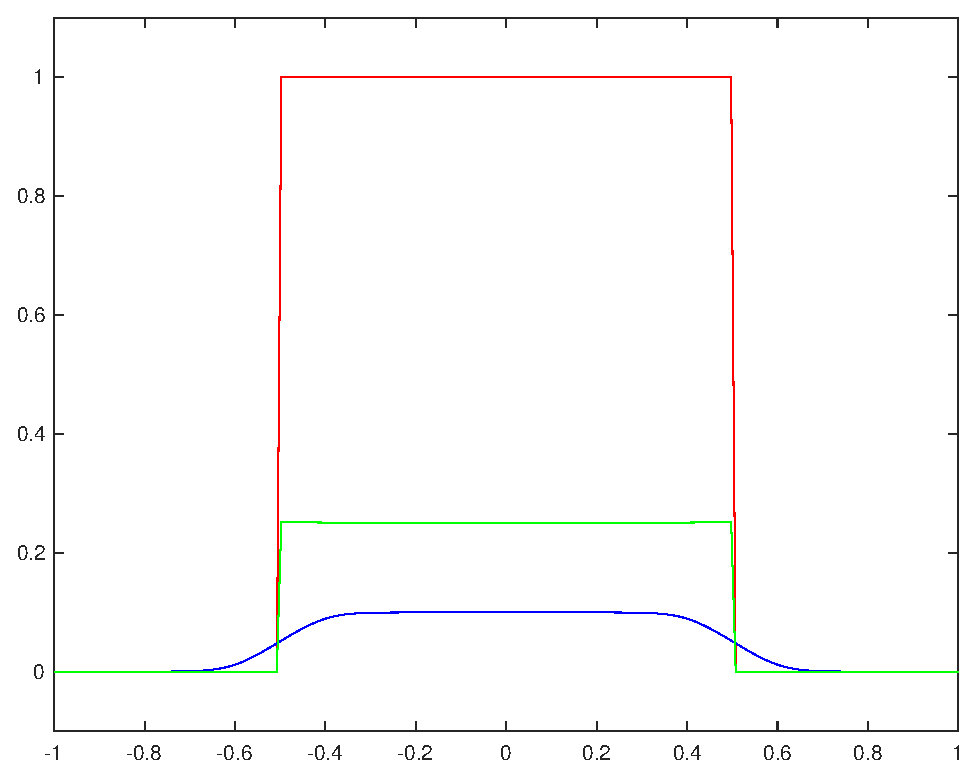
\includegraphics[width=0.4\textwidth]{Rectan.eps}
	\end{center}
	\caption{Benadering van de rechthoekige puls.}
	\label{fig:rectan}
\end{figure}

\begin{figure}[H]
	\begin{center} 
		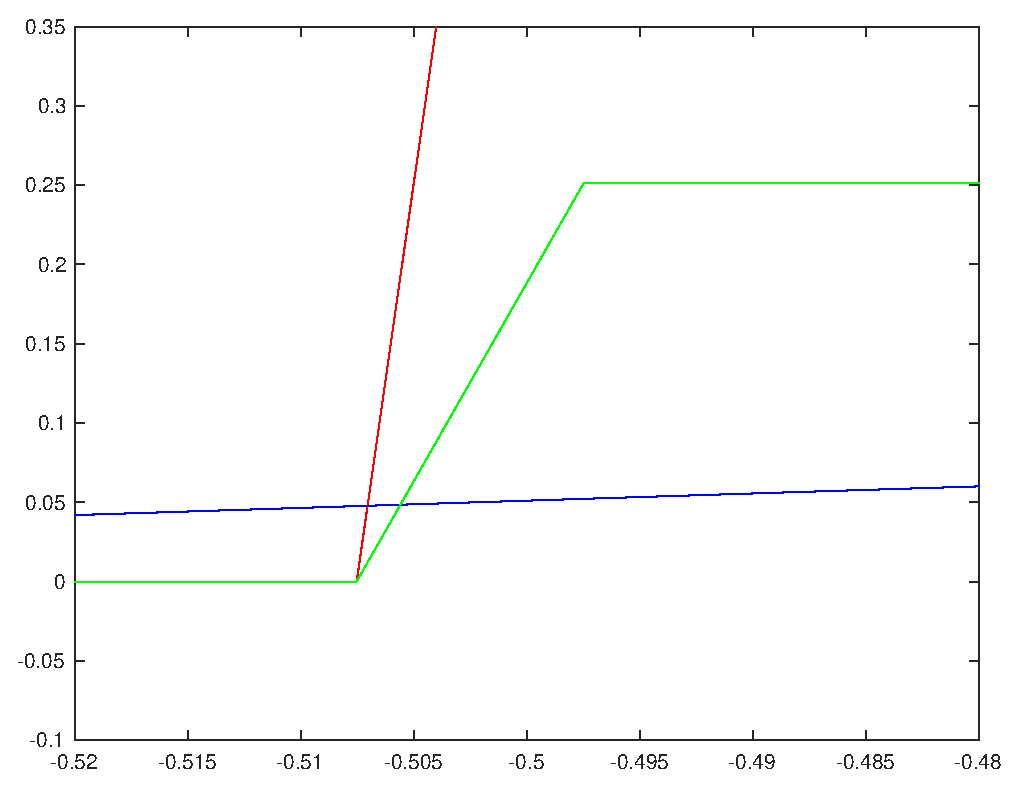
\includegraphics[width=0.4\textwidth]{RectanZoom.eps}
	\end{center}
	\caption{Benadering van de rechthoekige puls.}
	\label{fig:rectanZoom}
\end{figure}
\newpage

% OPGAVE 7
\opgave{7: Ruis}\label{sec:oef7}
De ruis wordt gemodelleerd aan de hand van (\ref{eq:f}) waaraan een willekeurige component wordt toegevoegd (\ref{eq:noise}).
\begin{equation}\label{eq:f}
	f(x) = \frac{\sin{(20x)}}{100x^2+5}
\end{equation}
\begin{equation}\label{eq:noise}
	f_{ruis}(x) = \frac{\sin{(20x)}}{100x^2+5} + 0.04*randn(size(x))
\end{equation}

Het minimale residu van de benaderingen wordt weergegeven in tabel \ref{tab:splineError}.
%Tabelletje
\begin{table}[H]
	\centering
	\begin{tabular}{l c r}
		Functie & Minimaal residu & Aantal knooppunten \\ \hline
		f(x) & 0.3380 & 199 \\
		Fruis(x) & 0.3469 & 190 \\
	\end{tabular}
	\caption{Optimaal residu en aantal knooppunten}
	\label{tab:splineError}
\end{table}

In figuur \ref{fig:errorkkb} werd norm(f\textsubscript{ruis} - z) (blauw) en norm(f - z) (rood) uitgezet in functie van het aantal equidistante knooppunten, met z de kkb van f\textsubscript{ruis}. Hierin is er een minimum, die, zoals reeds vermeld, in tabel \ref{tab:splineError} staan. In figuur \ref{fig:plotNoNoise} staan f(x) (rood) en de kkb van f(x) (blauw) geplot. In figuur \ref{fig:plotNoise} staan f\textsubscript{ruis}(x) (rood) en de overeenkomstige kkb (blauw). De figuren tonen ook aan dat de grootste benaderingsfouten zich voordoen waar de functie het meest varieert, zoals verwacht. Dit kan verholpen worden door in plaats van equidistante knooppunten, de knooppunten beter te verdelen in de buurt van de variaties. Dit kan echter enkel in de functie waar nog geen ruis aanwezig is, aangezien de variaties door ruis niet voorspelt kunnen worden. \\

\begin{figure}[H]
	\begin{center} 
		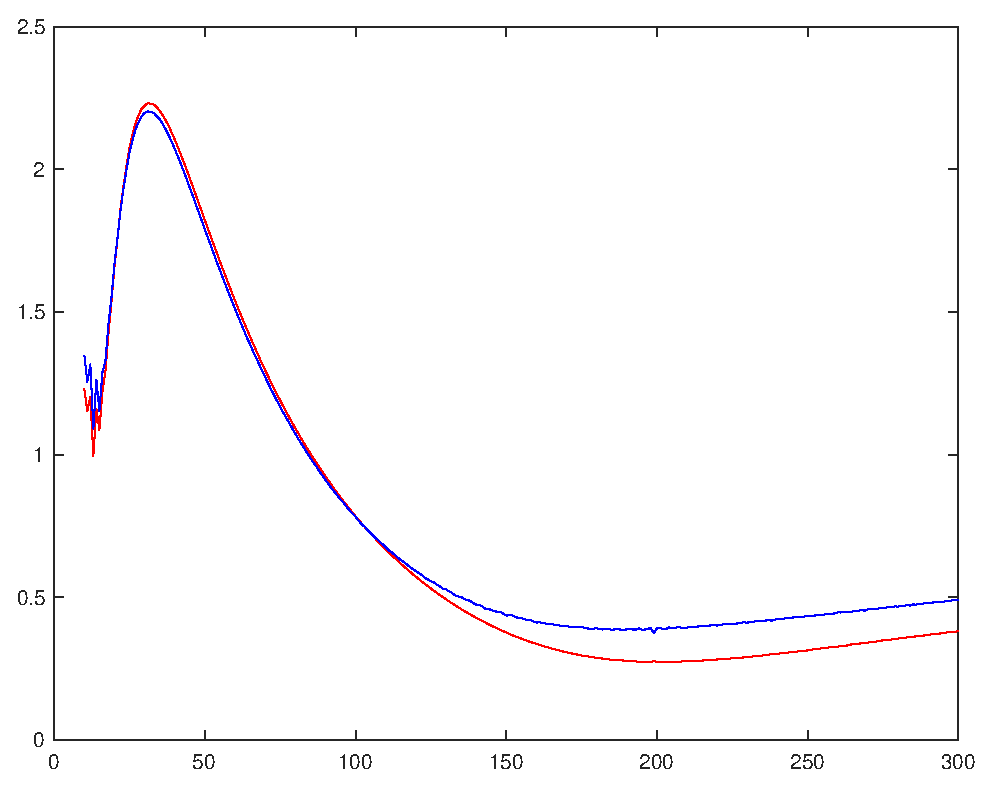
\includegraphics[width=0.4\textwidth]{ErrorBSplines.eps}
	\end{center}
	\caption{Fouten van de KKB implementatie.}
	\label{fig:errorkkb}
\end{figure}

\begin{figure}[H]
	\begin{center} 
		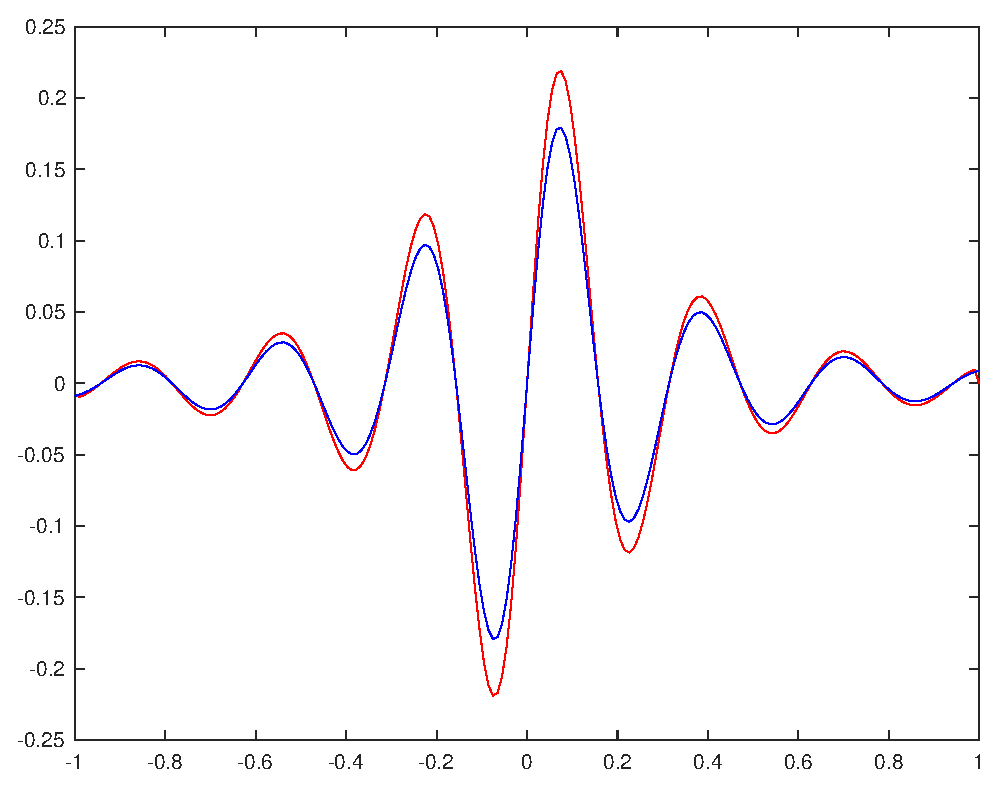
\includegraphics[width=0.4\textwidth]{PlotSplinesNoNoise.eps}
	\end{center}
	\caption{De functie f zonder ruis (rood) en beste benadering (blauw).}
	\label{fig:plotNoNoise}
\end{figure}

\begin{figure}[H]
	\begin{center} 
		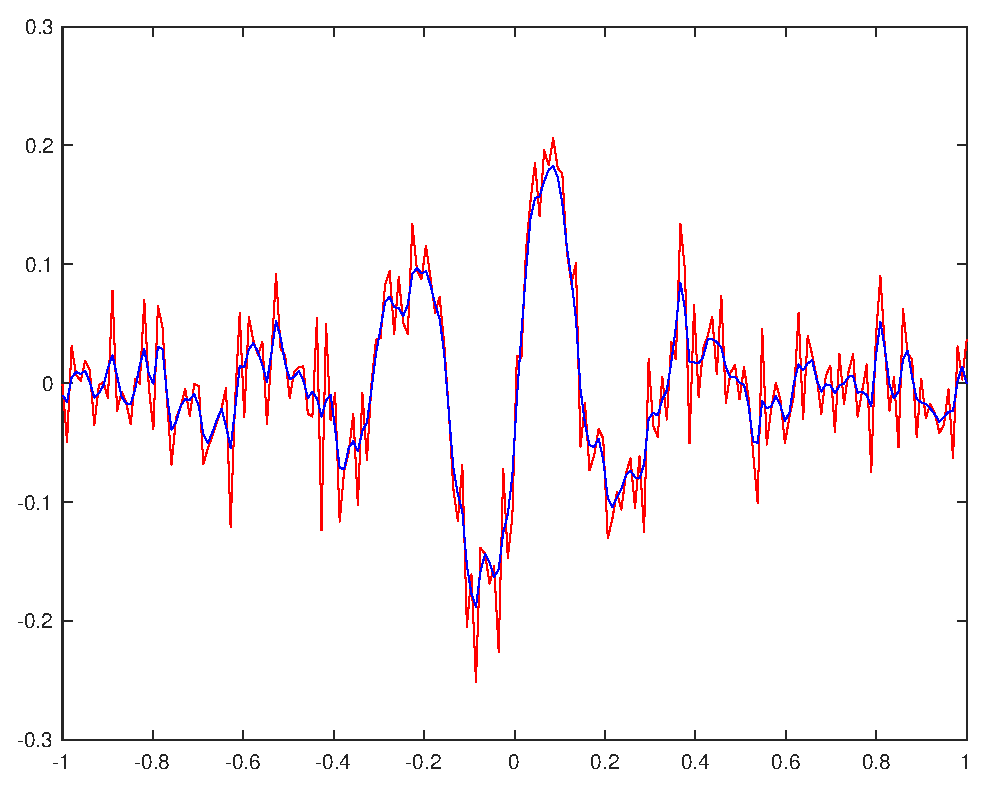
\includegraphics[width=0.4\textwidth]{PlotSplinesNoise.eps}
	\end{center}
	\caption{De functie f met ruis (rood) en beste benadering (blauw).}
	\label{fig:plotNoise}
\end{figure}

\end{document}